\chapter{OpenCAL OpenCL version}\label{ch:opencal-cl}

The goal of this chapter is to introduce to the user how to programme CA (Cellular Auto-
mata) with OpenCAL-CL (an extention of OpenCAL). OpenCAL-CL has
various benefit, infact it allows the user to execute your CA in a very easy
way on GPGPU through the OpenCL framework. OpenCL standard was
initially developed by Apple Inc. after it submitted this initial proposal
to Khronos Group. The main advantage of OpenCL is the portability. You can
execute your program whereever you want. You can execute across hetero-
geneous platforms consinsting of central processing units (CPUs), graphics
processing units (GPUs), digital signal processors (DSPs), field-programmable
gate arrays (FPGAs) and other processors. For this framework OpenCL a
more suitable motto might be, ''write once, run on anything''.\\
As previously mentioned OpenCAL-CL is an extention of OpenCAL (Open
Cellular Automata Library). 
OpenCAL-CL absorbs all the properties of
OpenCAL library moreover it adds parallel computation. Nowadays parallel 
computing is the best solution to cross temporal limits.
The AC definition in the host side is equals to the definition with the Open-
CAL library. However, the elementary process and other function of the
execution loop must be implemented as kernels. So one prerequisite to program 
 	with OpenCAL-CL is that the user must know OpenCL framework
to write kernels. On the other hand the library hide all things that the user
must not know, like execution loop is internal managed and the user can
set some properties about execution through some functions. Another thing
that it’s very boring in OpenCL and that the user must not do, it’s the data
transfer from host to kernel and vice versa because the user must call only
one easy function. So OpenCAL-CL library has the aim to simplify the user
prommaning. This book is divided into two parts. The first part focuses on
exploring the framework OpenCL and its capabilities. The second part
exploring the OpenCAL-CL library with some example to understand better the features of the library.

\section{OpenCL framework}
OpenCL enables parallel programming that assigns computational tasks to multiple processing elements 
to be perfomed at the same time. These tasks are called kernels. The kernel is a special function that can be executed 
to different OpenCL-compliant devices. The kernels are sent to the devices or device by host application.
The host application is a C/C++ application running on the user's system, called host.
The host application manage all the connection with devices by a container called context. 
In the host application, the user can select the kernel's functions to insert inside a container called program.
The program connects the kernel with argument data and dispaches it to a structure called command queue.
The command queue is a structure that allows the host to decide what the devices have to do, and when a kernel is enqueued, the device 
will execute the relative function.

\begin{figure}[htp]
  \begin{center}
    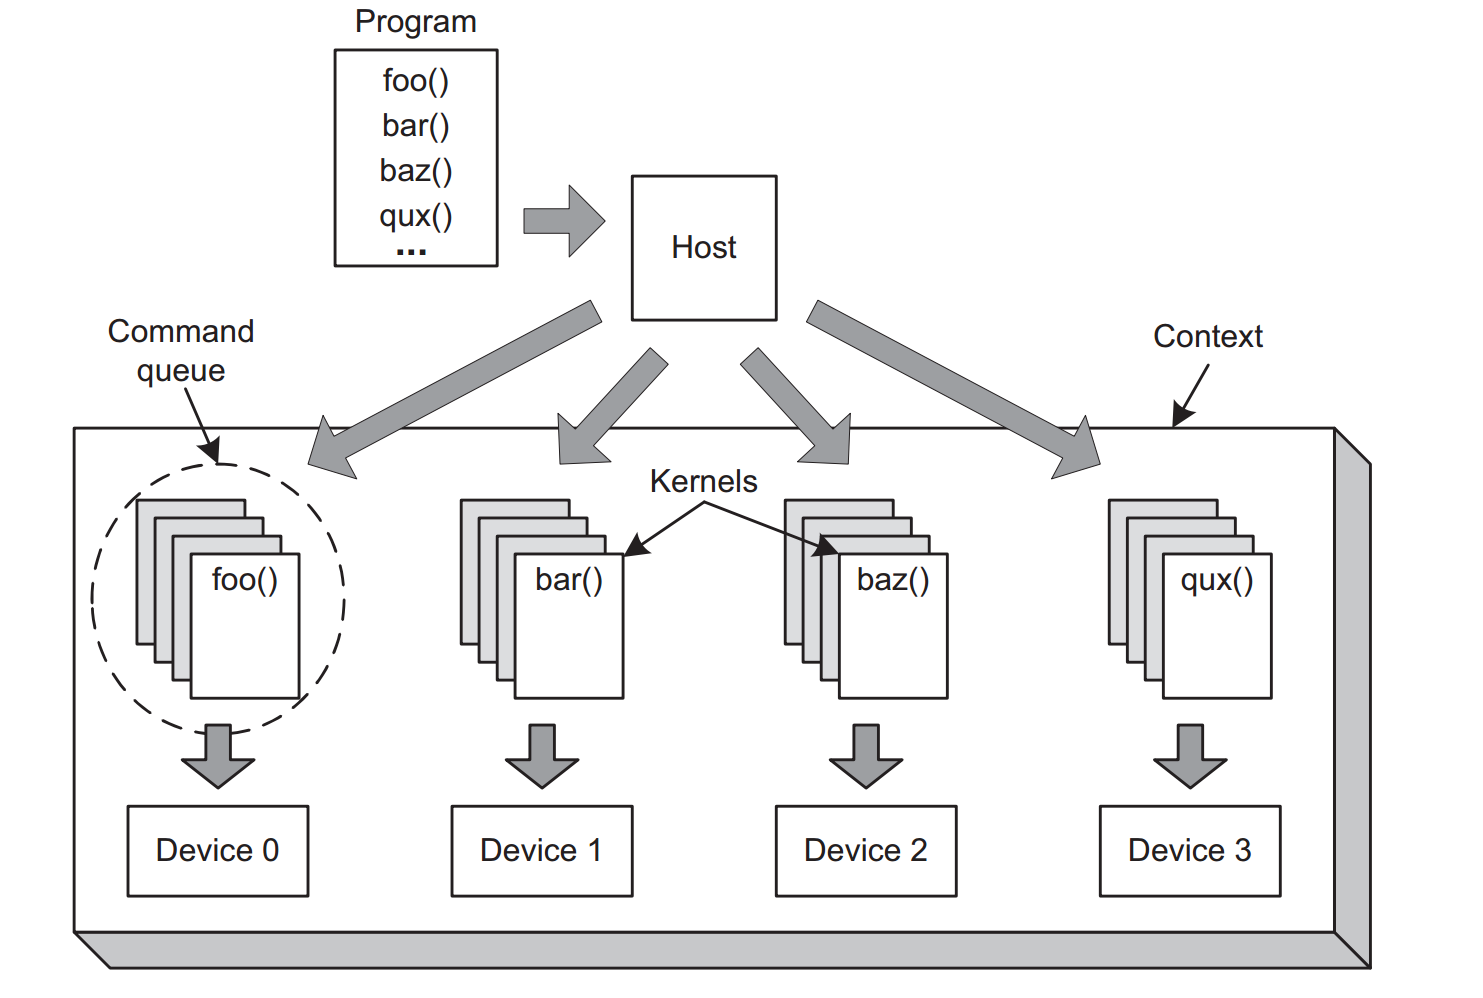
\includegraphics[width=12cm]{./images/OpenCAL-CL/kernelDistribution.png}
    \caption{General structure of a OpenCL program}
    \label{fig:GeneralStructure}
  \end{center}
\end{figure}

As we can see from the picture above, the context contains all the devices, all the command queues and all the kernels.
More in details, for every device is associated a command queue and every command queue has inside all the kernel functions
that the device has to execute.

\section{The structure of OpenCAL-CL}
As each OpenCL applications, the library OpenCAL-CL has a set of structures and
functions to develop host program and to define kernels. The definition of the
CA is specified in the host program. The user can define two type of model 2D or
3D, as shown in \ref{ch:opencal}. 
The host program manages the kernels and dispatches the data of the model, like (substates, type of neighbourhood, 
size of the cellular space,\ldots)
to the computation units.
The host program
manages the execution loop and which computation unit has to execute the
transaction functions. \\
The host program is divided in the follows sections:
\begin{itemize}
\item definition of the model (Chapter \ref{ch:opencal}) 
\item manage of the devices OpenCL
\item allocation of kernels
\item send data from the model to devices
\item start execution loop
\end{itemize}

\section{Host programming} 

\subsection{Manage of the devices}

After we created the model, the user must choose the device for the computation.
Inside the library there is a structure called CALOpenCL that allows the user to manage all 
available platforms and devices.
This structure simplifies the access to the devices compared with the native API
of OpenCL. The library supplies other function to know which platforms and
devices are available on the system and to have information about these.\\
Below you can see a simply program explains how the structure
CALOpenCL can be used.


\begin{lstlisting}
#include <calCL2D .h>

 int main (){

 CALOpenCL * calOpenCL = calclCreateCALOpenCL ();
 // get all available platforms
 calclInitializePlatforms ( calOpenCL );
 // get all available devices
 calclInitializeDevices ( calOpenCL );

 // get the first device on the first platform
 CALCLdevice device = calclGetDevice ( calOpenCL , 0, 0);

 // create a context
 CALCLcontext context = calclcreateContext (& device , 1);

 return 0;
 }
\end{lstlisting}

Inside the library, the platforms and the devices are store in a matrix where the
rows represent the platforms and the columns represent the devices. So to choose which one we can use for the computation,
it's necessary specify the index of platform and the index of the device. For
example, at lines 12, we chose the platform number
0 and the device number 0. If we have an system with 3 GPUs NVIDIA and 3 GPUs
AMD, the library will have a matrix with size 2x3 where 2 are the
vendors(the platforms NVIDIA and AMD) and 3 are the GPUs for each platforms.If we want to 	
run the program to the third AMD GPU we can specify as indices 1 and 2.
If we don't know how the system identify the platforms and devices, the
library give us a function called \verb'calclGetPlatformsAndDeviceFromStandardInput'
the allows us to know the platforms and device. First it prints the
information on standard output and then we can insert the indexes directly from
standard input.\\
After we chose the device, the user must specify the path where are the kernels
and relative headers.
Through the function \verb'calclLoadProgramLib(2D/3D)' the library reads automatically
the kernels and compiles their.
\begin{lstlisting}
CALCLprogram calclLoadProgramLib(2D|3D) ( CALCLcontext context ,
CALCLdevice device , char * path_user_kernel , char *
path_user_include )
\end{lstlisting}

\subsection{Allocation of kernels}

The library doesn't know which kernels they have to run, for this reason the
user must specify the names of the kernels.
To create and allocate a kernel it's necessary to call the function
\verb'calclGetKernelFromProgram' that gets an OpenCL kernel given a compiled OpenCL
program. 

\begin{lstlisting}
cl_kernel elementaryProcess = calclGetKernelFromProgram(&program,
KERNEL_NAME);
\end{lstlisting}


\subsection{Send data from the model to devices}

To transfer the data from host side to kernel side, in the library, there is
a structure called \verb'CALCLToolkit(2D/3D)' contains all the buffers object of the
model and all the buffers object of the library. 
By default the library sends to all the kernels the data belongs to the model. The following list shows the
data sended:
\begin{itemize}
	\item the dimension of cellular space 
	\item the number of substate for every type (byte,int,real) 
	\item the substates allocated from the user
	\item the list of active cells
	\item the list of active cells flags
	\item type, dimension and ID of the neighbourhood
	\item the border condition
\end{itemize}


 First the user must create an
instance of the structure \verb'CALCLToolkit(2D/3D)' through calling the function
\verb'calclCreateToolkit' as shown the following code
\begin{lstlisting}
CALCLToolkit2D * calclCreateToolkit (2D|3D)(struct CALModel (2D|3D) *model ,CALCLcontext context ,CALCLprogram
program ,CALCLdevice device ,CALCLOptimization opt)
\end{lstlisting}
The enumerative \verb'CALCLOptimization' allows the user to choose if it wants to use
the library without optimization \verb|(CALCL_NO_OPT)| or with active cells optimization
 \verb|(CALCL_OPT_ACTIVE_CELLS)|. The structure \verb'CALCLToolkit(2D/3D)'
doesn't contain only the buffers to transfer data but also the kernels belong to the
excution loop. \\
To add a new kernel to the execution loop the user have to call the function \verb'calclAddElementaryProcessKernel(2D/3D)' that
adds the chosen kernel to the list of elementary processes moreover it sends to
the device all the necessary data to execute the kernel.

\begin{lstlisting}
void calclAddElementaryProcessKernel2D(CALCLToolkit2D * toolkit2d, struct CALModel2D *model, CALCLkernel * kernel);
\end{lstlisting}


\subsection{Start execution loop}

To start the execution loop the user have to call the function \verb'calclRun(2D/3D)'. The function executes
all the elementary processes previously declared on the specified device.

\begin{lstlisting}
void calclRun2D(CALCLToolkit2D* toolkit2d, struct CALModel2D * model, unsigned int initialStep,	unsigned maxStep);
\end{lstlisting}


\section{Kernel programming} 

As in the host programming, in the kernel programming the user can use some functions
to simply the interaction with the data structures. These functions are available inside \verb'cal2D.h' or \verb'cal3D.h'.
These functions are the same host features, the only difference is the first parameter. Infact the host to use this key word 
\verb'MODEL_DEFINITION2D' that defines the model parameters.


The code below shows how to declare a new kernel.

\begin{lstlisting}
__kernel void sciddicaTSteering(MODEL_DEFINITION2D)
\end{lstlisting}


On the GPU side, the user has to create a file that contains the kernels  



